\documentclass [a4paper, 11pt] {article}

%packages
\usepackage [english] {babel}
\usepackage [T1] {fontenc}
\usepackage [utf8] {inputenc}
\usepackage {graphicx}
\usepackage {subcaption}
\usepackage {amsmath}
\usepackage {amssymb}
\usepackage {amstext}
\usepackage {amsthm}
\usepackage {listings}
\usepackage {tikz}
\usepackage[
pdftex,
pdfauthor={Goxhufi, Driton; Ravlija, Damir},
pdftitle={MLGV - Exercise 1 Submission},
pdfsubject={Machine Learning in Graphics \& Vision Homework}
]{hyperref}

\usepackage[a4paper,lmargin={2cm},rmargin={2cm},tmargin={3.5cm},bmargin = {2.5cm},headheight = {4cm}]{geometry}

\usepackage[shortlabels]{enumitem}
\usepackage{lastpage}
\usepackage{fancyhdr}

\usepackage{lipsum}
\usepackage{ifthen}

\pagestyle{fancy}

%document configuration
\newcommand{\courseName}{Machine Learning in Graphics \& Vision}
\newcommand{\termYear}{Summer Term 2020}
\newcommand{\homeworkNum}{1}
\newcommand{\studentOne}{Driton Goxhufi}
\newcommand{\studentTwo} {Damir Ravlija}
\newcommand{\matrikelNrStOne}{4233242}
\newcommand{\matrikelNrStTwo}{5503184}
\newcommand{\mailStOne}{driton.goxhufi@student.uni-tuebingen.de}
\newcommand{\mailStTwo}{damir.ravlija@student.uni-tuebingen.de}

%other config
\renewcommand{\vec}[1]{\boldsymbol{#1}}
\newcommand{\mat}[1]{\boldsymbol{#1}}
\newcommand{\m}[1]{\begin{pmatrix}#1\end{pmatrix}}
\newcommand{\tr}[2]{{}^{#1}T_{#2}}
\graphicspath{{./images/}}


\lhead{\begin{tabular}{l}
		\courseName\\
		\termYear \\
		Exercise \homeworkNum
\end{tabular}}
\rhead{\begin{tabular}{lr}
		\studentOne & \matrikelNrStOne \\
		\studentTwo & \matrikelNrStTwo \\
\end{tabular}}

\begin{document}
	
\title{\vspace{-1.5cm}\textbf{Exercise \homeworkNum} \\ 
	\courseName}
\author{\begin{tabular}{lcr}
		\studentOne & \matrikelNrStOne & \href{mailto:\mailStOne}{\mailStOne} \\
		\studentTwo & \matrikelNrStTwo & \href{mailto:\mailStTwo}{\mailStTwo} 
\end{tabular}}	
\date{}
\maketitle


\section{Task 1}

\begin{enumerate}
	\item[(a)] The complexity of the method in subtask (a) is $O(d*n^2)$ where $d$ is the dimension of feature vector and $n$ is the number of examples. Plot of the results in figure \ref{fig:1a}).
	
	Code in \texttt{problem\_1\_1\_a\_b.py}.
		
	\item[(b)] A single vector has to be compared with \\
	$30$ FPS $* 120$ s $= 3,600$ frames $= 3,600 * 20,000 = 7.2 * 10^7 (\text{or } 3,600N)$ vectors \\
	in one video, and each one of these has to be compared with all of the vectors from another video (i.e. $7.2 * 10^7 (\text{or } 3,600N)$ vectors as well).\\
	There are therefore $128 * {7.2}^2 * 10^{14} (\text{or } 128 * (3,600N)^2$ comparisons. Assuming that the machine can compute $3 * 10^9$ comparisons in a second, it would take $221,184,000$ s $\approx 7.0137$ years or $(0.55296 N^2 \text{ seconds})$ to find all matchings of the vectors between two different 2 minute long videos ($30$ FPS) using \texttt{exhaustive\_search}.
	
	Code in \texttt{problem\_1\_1\_a\_b.py}. Plot of the results in figure \ref{fig:1b}).
	
	\begin{figure}[!h]
		\centering
		\begin{subfigure}{0.4\textwidth}
			\centering
			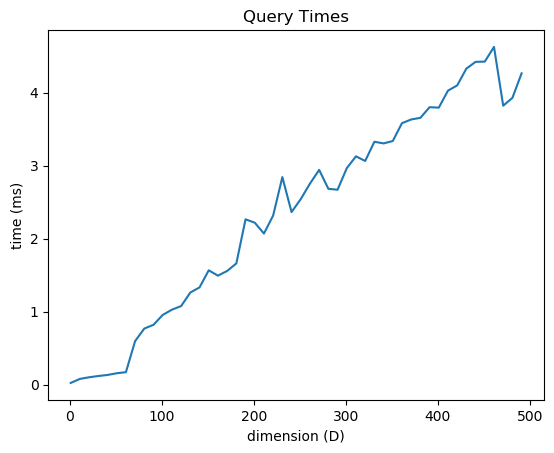
\includegraphics[width=\textwidth]{1_1_a.png}
			\caption{}
			\label{fig:1a}
		\end{subfigure}
		\begin{subfigure}{0.4\textwidth}
			\centering
			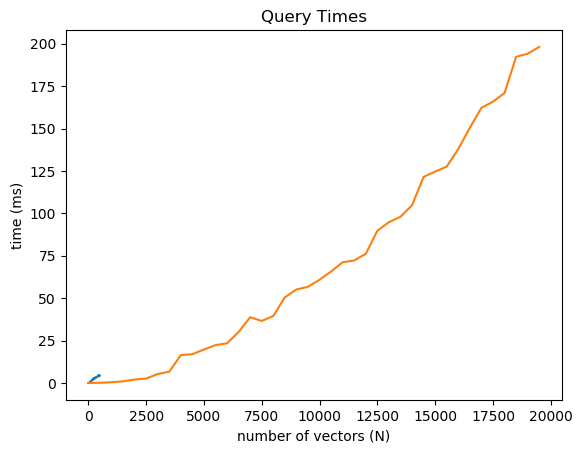
\includegraphics[width=\textwidth]{1_1_b.png}
			\caption{}
			\label{fig:1b}
		\end{subfigure}
		\begin{subfigure}{0.4\textwidth}
			\centering
			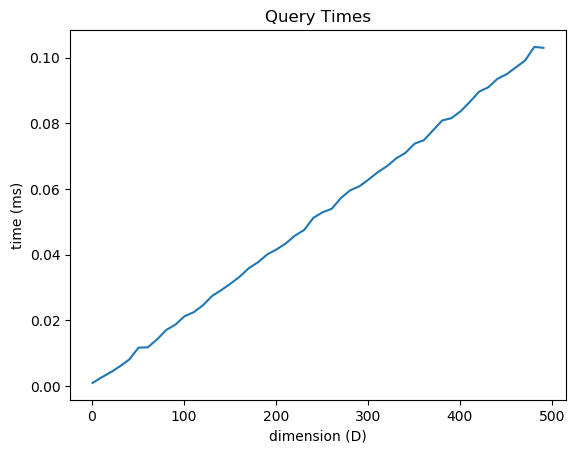
\includegraphics[width=\textwidth]{1_1_c.png}
			\caption{}
			\label{fig:1c}
		\end{subfigure}
		\caption{Plot of results from task 1}
		\label{fig:1}
	\end{figure}

\item[(c)]
	Query times in both, exhaustive and KDTree search grow linearly as the number of dimensions increases. However, KDTree is us for datasets with more dimensional vectors up more than $20$ times faster. This implies that another variable, the number of vectors in the dataset, is the source of this difference. 
	
	Code in \texttt{problem\_1\_1\_c.py}. Plot of the results in \ref{fig:1c}
	
\end{enumerate}	

\section{Task 2}
\begin{enumerate}
	\item[(a)] Code in \texttt{problem\_1\_2\_a.py}. Top-K accuracy for $K$ between $1$ and $10$ as expected grows with $K$ and is in the range between $0.8$ and $0.97$ (Figure \ref{fig:2a}).
	\begin{figure}[!h]
		\centering
		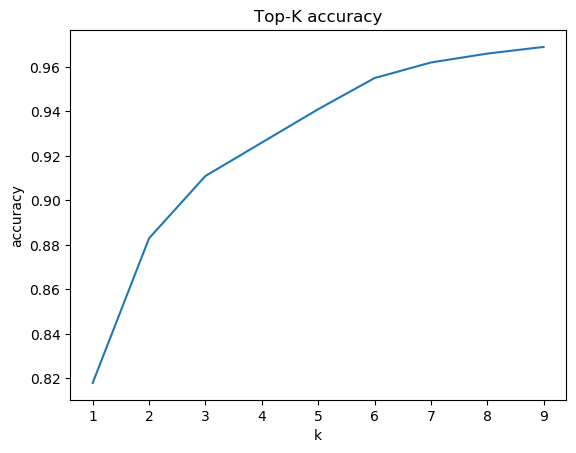
\includegraphics[width=0.5\textwidth]{1_2_a.png}
		\caption{Top-K accuracy for $K = 1, 2,\dots, 10$ using the KD-tree}
		\label{fig:2a}
	\end{figure}

	\item[(b)]	Code in \texttt{problem\_1\_2\_b.py}.
	
	Obtained results:
	\begin{lstlisting}[mathescape=true]
Precision (with "Pullover" (2) as positive):  0.8333333333333334
Precision (with "Shirt" (6) as positive):  0.780952380952381
------------------------------------------------------------
Recall (with "Pullover" (2) as positive):  0.7653061224489796
Recall (with "Shirt" (6) as positive):  0.845360824742268
	\end{lstlisting}
	
\end{enumerate}
	
	
	

	
\end{document}

